% id: 0391
% book: 쎈 중3-2 수학 · 03 원과 직선
% section: C단계 만점 도전하기 · 서술형
% figure: tikz:fig-0391
% answer: $\left(16\sqrt{3}-\dfrac{16}{3}\pi\right)\mathrm{cm}^2$
% answer_source: 답지
% variant_level: 0 (원본 전사)
% 이 파일은 build.mjs 가 items.json 에서 만든다. 고칠 때는 items.json 을 고친다.
\smash{\raisebox{1.5mm}{\dmkichul{쎈 중3-2 수학 0391번 · 73쪽}}}
\noindent\begin{minipage}[t]{0.58\linewidth}\vspace{0pt}\raggedright 오른쪽 그림과 같이 점~$\pt{P}$에서 원~$\pt{O}$에 그은 두 접선의 접점을 $\pt{A}$, $\pt{B}$라 하자. $\seg{OA}=4\,\mathrm{cm}$이고 $\angle\pt{APB}:\angle\pt{AOB}=1:2$일 때, 색칠한 부분의 넓이를 구하시오.\end{minipage}\hfill\begin{minipage}[t]{0.4\linewidth}\vspace{0pt}\centering \resizebox{\ifdim\width>\linewidth\linewidth\else\width\fi}{!}{% 0391(본책 73쪽) — 점 P 에서 원 O 에 그은 두 접선(접점 A, B), OA=4 cm, ∠APB:∠AOB=1:2, P 와 호 AB 사이 색칠. 답(넓이)은 적지 않는다. 스캔 삽화를 TikZ 로 다시 그림.
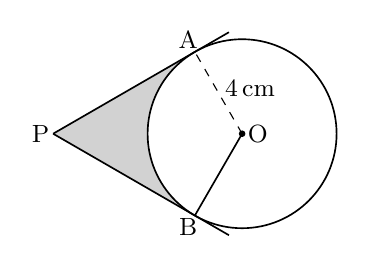
\begin{tikzpicture}[line width=0.6pt]
  \fill[gray!35] (-2.400,0.000) -- (-0.600,1.039) arc[start angle=120, end angle=240, radius=1.200cm] -- cycle;
  \draw (0.000,0.000) circle (1.200);
  \fill (0.000,0.000) circle (1.2pt);
  \draw (-2.400,0.000) -- (-0.167,1.289);
  \draw (-2.400,0.000) -- (-0.167,-1.289);
  \draw[dashed, line width=0.4pt] (0.000,0.000) -- (-0.600,1.039);
  \draw (0.000,0.000) -- (-0.600,-1.039);
  \node[font=\small, inner sep=1.5pt] at (0.100,0.570) {$4\,\mathrm{cm}$};
  \node[font=\small, inner sep=1.5pt] at (-0.685,1.186) {A};
  \node[font=\small, inner sep=1.5pt] at (-0.685,-1.186) {B};
  \node[font=\small, inner sep=1.5pt] at (-2.560,0.000) {P};
  \node[font=\small, inner sep=1.5pt] at (0.200,0.000) {O};
\end{tikzpicture}
}\end{minipage}\par
